\documentclass[conference]{acmsiggraph}

% http://en.wikibooks.org/wiki/LaTeX/Algorithms
\usepackage{algorithm2e}
% \usepackage{algpseudocode}

\usepackage{float}
\usepackage{caption}
\usepackage{amsmath}
\usepackage{url}
\usepackage{hyperref}

\newcommand\blfootnote[1]{%
  \begingroup
  \renewcommand\thefootnote{}\footnote{#1}%
  \addtocounter{footnote}{-1}%
  \endgroup
}

\TOGonlineid{45678}
\TOGvolume{0}
\TOGnumber{0}
\TOGarticleDOI{1111111.2222222}
\TOGprojectURL{}
\TOGvideoURL{}
\TOGdataURL{}
\TOGcodeURL{}

\title{Chronographer - A Location History Visualization Tool}


\author{Scott Todd\thanks{email: todds@rpi.edu}}
\pdfauthor{Scott Todd}

\keywords{Data Visualization, Geographic Data, Virtual Reality}

\begin{document}

\teaser{
    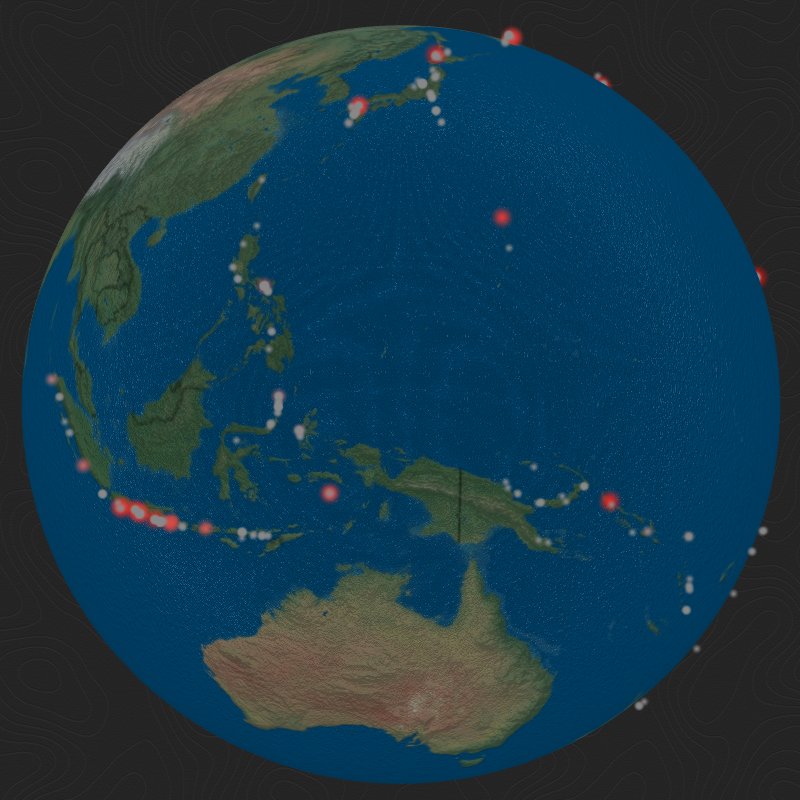
\includegraphics[height=180px]{images/chronographer.png}
    \captionsetup{hypcap=false}
    \caption{Visualizing volcanic eruptions}
}

\maketitle


\begin{abstract}

I created a geographic location history visualization tool titled Chronographer
that explores virtual reality interaction as a data analysis aid. I used
three.js \cite{three.js}, the device orientation API
\cite{Mozilla:DeviceOrientation}, and the Google Cardboard
\cite{Google:Cardboard} viewer to construct this visualization, which is hosted
at \url{http://scotttodd.github.io/Chronographer/}. I visualized location
history data exported from my Google account using Google Takeout
\cite{Google:Takeout} as well as volcanic eruption data from NOAA
\cite{NOAA:Volcano}. I went through several design iterations and concluded that
this style of visualization is interesting but not currently effective as a
tool for learning from geographic data sets. I conducted informal user testing
partway through the project but did not perform a rigorous user study.

\end{abstract}

\keywordlist

\TOGlinkslist

%% Required for all content.
\blfootnote{Project Repository: https://github.com/ScottTodd/Chronographer}

\copyrightspace


\section{Introduction}

Geographic location history data sets combine spatial information which demands
context with chronological information which benefits greatly from interaction
or animation. Existing map-based tools present geographic data in an
understandable format but they each rely on a projection that introduces an
extra level of processing in order to relate the data to the physical world.
Virtual reality has been growing in popularity and technical maturity in recent
years and offers the opportunity to connect people to data in ways not possible
before. I wanted to test the utility of virtual reality in helping people
understand these data sets.

The representation of the time axis is also important for data analysis.
Several techniques have been researched in the past which handle user control
over the time axis differently.

Virtual reality devices such as the Oculus Rift and Sony's Project Morpheus are
currently in active development. Screen, positional tracking, and rendering
technologies have advanced to the point where immersive virtual reality is
nearly within reach for consumer-grade projects. The Google Cardboard takes a
step in a different direction and leverages current generation smart phones,
which are packed with sensors and high resolution screens already, to deliver an
affordable virtual reality solution that hobbyists and consumers can easily use.

Virtual reality for web browsers is a recent extension of these new
technologies, so support and stability are both limited. The device orientation
API is experimental and has several shortcomings, but it may eventually be
replaced with official browser support through a technology currently being
named WebVR.


\subsection{Related Work}

\subsection{Technical References}

``What is Spatial History'' by Richard White \cite{White} details efforts to
chronicle history through data visualization, making sense of large data sets
through visual media, rather than through words alone as traditional history
textbooks do. He argues that spatial relations are established through movement
- movement of people, goods, and information. He discusses
``relational space'', where locations are closer at different points during a
day due to traffic and other relative, modern factors. He also concludes that
visualizations are a means of doing research and generating questions that may
have otherwise gone unasked, not a method to communicate findings discovered
through other means.

The DimpVis system \cite{10.1109/TVCG.2014.2346250} explores a novel method of
interacting with data points on two-dimensional plots with time as a third
axis. Where time is normally controlled by a slider, it allows for users to
drag points along hint paths to move through time in either direction.

\subsection{Further Inspiration}

GitHub user @theopolisme created a website that lets you visualize your Google
Location History using an interactive heatmap
\cite{location-history-visualizer}. In his visualization, data points from all
time values are compressed onto a single map which features zoom and pan
controls.

A blog post titled ``Virtual Reality brings Big Data visualization to life''
by Mike Wheatley \cite{VR:BigData} argues that good data visualization tools
should consider human visual perception and give insight into the unknown, not
the already-understood. It explains how DARPA used the Oculus Rift to visualize
three-dimensional network simulations and how engineers at Caltech used virtual
worlds such as Second Life and the Unity3D game engine as data visualization
platforms.


\section{Datasets and Data Collection}

I used my personal location history data collected via Google Takeout, which is
formatted as a simple JSON file containing an array of [latitude, longitude,
timestamp] triples. This data file is 76 MB in size and contains nearly 420,000
data points collected between 2013 and 2014.

I also visualized the history of volcanic eruptions using data from the NOAA
Significant Volcanic Eruptions Database. I coverted this data from a Microsoft
Excel file into the same JSON format that Google Takeout uses. While this data
set contains eruptions between the year -4000 and the present, I found that the
older data was too sparse and made navigation via the time slider difficult, so
I extracted only eruptions between 1800 and the present.

\section{Development}

\subsection{First Ideas}

I originally planned to build a two dimensional map interface that would blend
a set of data points across time ranges together. At this point, I was inspired
by @theopolisme's Location History Visualizer and had recently completed another
map-based visualization using d3.js \cite{D3.js}. Because of my familiarity with
d3.js and three.js, I hoped to combine the powerful WebGL rendering of three.js
with the convenient map projection and rendering of d3.js to visualize my own
location history. I had also been searching for a reason to experiment with the
Google Cardboard, so I worked that into my plans.

\subsection{Initial Implementation}

My basic visual design centered around displaying data points above a map and
using additive or alpha blending to show general regions where points were
focused. As the visualization time changed, data points would fade in and out.
I used a traditional slider to control the visualization time, which could be
set to play automatically or could be manually controlled via mouse or touch.
Next to the slider, I placed the current time and a play/pause button. This
initial design can be seen in Figure 2.

I used a particle system to represent data points, with each data point having
a single particle in the particle system to represent it. These particles would
change their display properties based on the difference between the
visualization time and their data point's time through computations in a set
of custom vertex and fragment shaders which render billboarded (always
camera-facing) particles (see Algorithm 1).

\RestyleAlgo{boxruled}
\begin{algorithm}
\DontPrintSemicolon
\caption{Data Point Rendering}
    \KwData{$visualizationTime$, $minTime$, $maxTime$, $highlightPercent$,
            transformation matrices}
    \ForEach{particle} {
        \KwData{$particleTime$, $latitude$, $longitude$}
        \begin{enumerate}
            \item Position in screen space based on $latitude$, \\
                $longitude$, and transformation matrices
            \item Compute $visPercent$ as the percentage that
                $visualizationTime$ is from $minTime$ to $maxTime$
            \item Compute $particlePercent$ as the percentage that
                $particleTime$ is from $minTime$ to $maxTime$
            \item Compute $percentDifference$ and scale by $highlightPercent$
            \item Interpolate HSV color, size, and alpha using this scaled
                percentage
            \item Draw particle image with computed properties
        \end{enumerate}
    }
\end{algorithm}

\begin{figure}
  \centering
  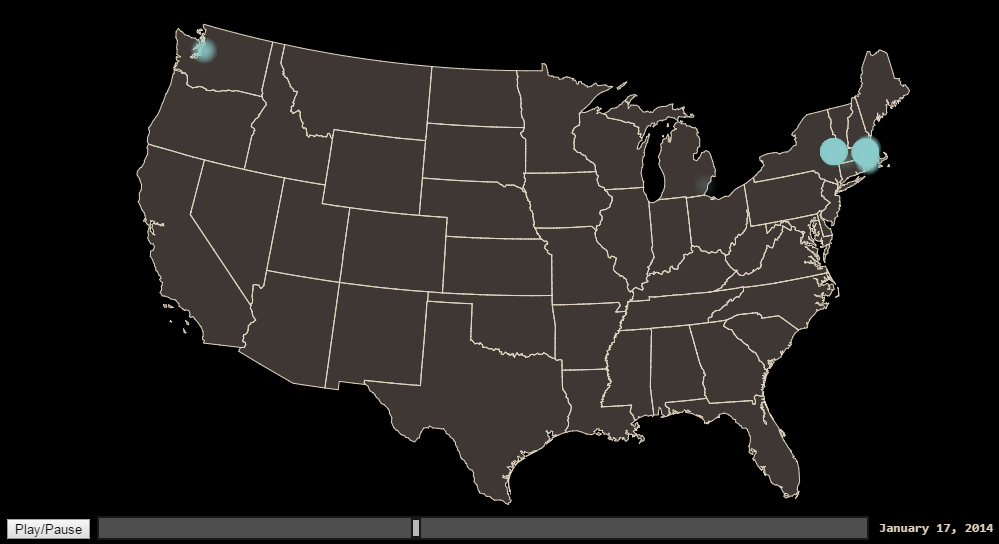
\includegraphics[width=3.4in]{images/initial_us_map}
  \caption{Initial map of the USA with data point particles. Note the slider at
           the bottom of the screen}
\end{figure}

\subsection{First Extensions}

After producing a working 2D implementation of my basic idea, I experimented
with other projections (Figures 3 and 4), eventually aiming for a spherical
projection that would have potential as an effective virtual reality view.

\begin{figure}
  \centering
  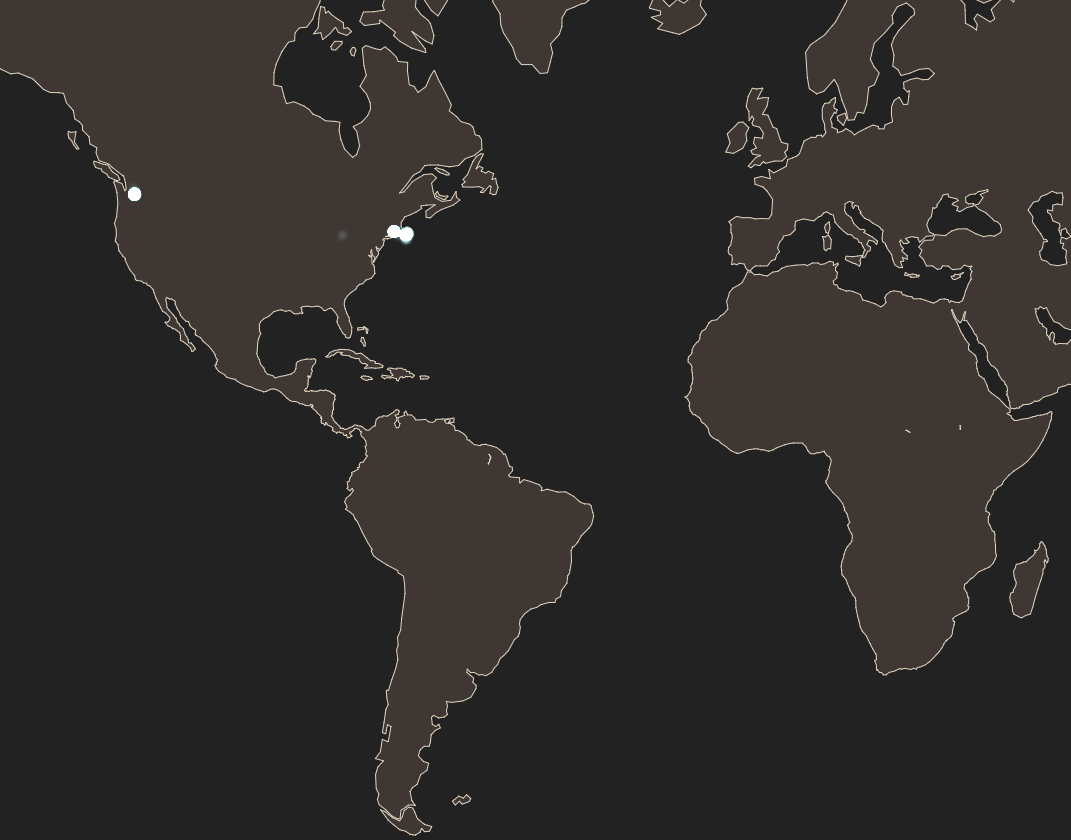
\includegraphics[width=3.0in]{images/mercator_projection_with_particles}
  \caption{Mercator projection with data point particles}
\end{figure}

\begin{figure}
  \centering
  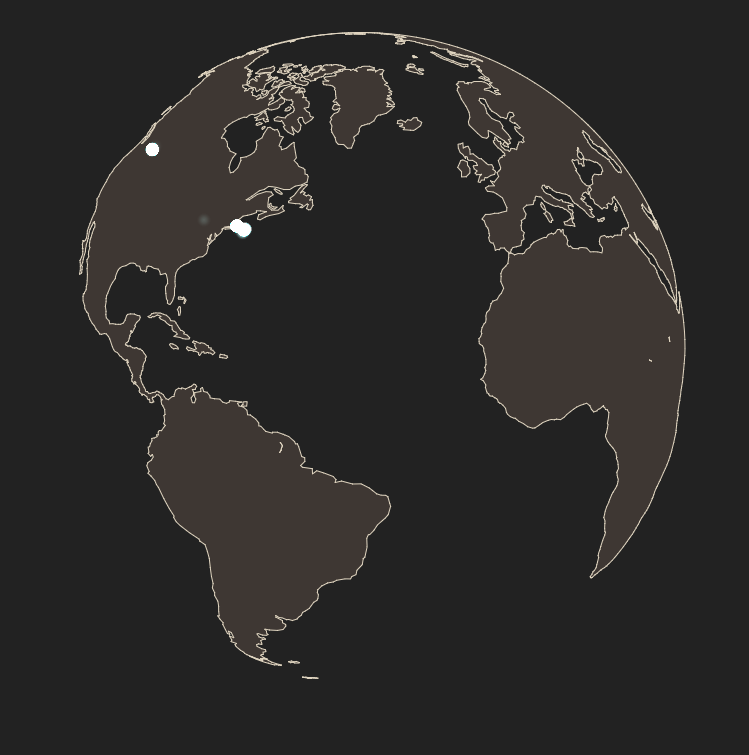
\includegraphics[width=3.0in]{images/orthographic_projection_with_particles}
  \caption{Orthographic projection with data point particles}
\end{figure}

Up until this point, I had been combining d3.js and three.js and used an awkward
bridge between them to reliably communicate the projection and viewport
information needed to render both a map and a particle system on the same
screen (see Algorithm 2). This algorithm required constant data processing, so
it acted as a bottleneck for my entire application. In order to render my
location history, I had to process through the data and discard all but 1 out of
every 100 data points. I realized that if I switched entirely to a spherical
projection, I could render the map using three.js rather than with d3.js,
removing the need to operate through that additional level of abstraction.

\RestyleAlgo{boxruled}
\begin{algorithm}
\DontPrintSemicolon
\caption{Initial Data Point Positioning}
    At load time : \ForEach{data point} {
        Create a particle in the particle system, storing latitude and longitude
    }
    At run time : \ForEach{frame} {
        \ForEach{particle} {
            \begin{enumerate}
                \item Convert from latitude/longitude to screen-space \\
                    {[}x, y{]} using d3.geo.projection
                \item Convert from screen-space {[}x, y{]} to three.js \\
                    world-space {[}x, y, z{]} using \\
                    THREE.Projector.unprojectVector
                \item Update {[}x, y, z{]} vertex position for this particle
            \end{enumerate}
        }
        Render all particles using the technique in (Algorithm 1)
    }
\end{algorithm}

\subsection{Moving away from d3.js}

I completely transitioned away from d3.js and rendered the Earth using a
textured sphere (Figure 5). I used a diffuse, specular, and bump map from a free
website. The bump map was roughly an elevation map of the world and the specular
map was roughly a water coverage map. My new data point positioning algorithm
using only three.js is outlined in Algorithm 3. With this new positioning,
the bottleneck that used to exist was resolved, so I could now render those
original 420,000 data points my location history file at 60 frames per second.

\RestyleAlgo{boxruled}
\begin{algorithm}
\DontPrintSemicolon
\caption{Updated Data Point Positioning}
    \KwData{radius}
    At load time : \ForEach{data point} {
        \begin{enumerate}
            \item Create a particle in the particle system
            \item Store latitude and longitude
            \item Convert latitude and longitude to object-space [x, y, z]
                \begin{enumerate}
                    \item $phi = latitude$, $theta = longitude$
                    \item $x = radius * cos(phi) * cos(theta)$
                    \item $y = radius * sin(phi)$
                    \item $z = radius * cos(phi) * sin(theta)$
                \end{enumerate}
        \end{enumerate}
    }
    At run time : \ForEach{frame} {
        Render all particles using the technique in (Algorithm 1)
    }
\end{algorithm}

\begin{figure}
  \centering
  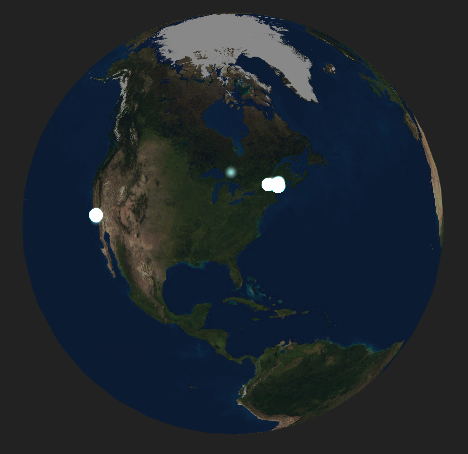
\includegraphics[width=3.0in]{images/threejs_sphere_earth}
  \caption{Sphere and particles rendered entirely with three.js}
\end{figure}

\subsection{Virtual Reality}

Virtual reality display and interaction were implemented as a secondary display
mode with the help of the device orientation API and stereo rendering effects.
The device orientation API exposes alpha, beta, and gamma values representing
the orientation of an input device in 3D space through the deviceorientation
JavaScript event. The meaning of these values seems to change based on the
layout of the device (portrait or landscape in the case of my phone), so I fixed
the layout to landscape mode using ``screen.orientation.lock()''. I used these
angle values to orbit the camera around the central world. In this way, users
can look around a virtual world centered in front of their phone.

My Samsung Galaxy S4 phone has several known issues with its magnetometer
(interference) and gyroscope (calibration), making integration with the Google
Cardboard unreliable. Newer phones suffer less from these issues though, as
these technologies become more well established. Additionally, web browsers are
known to send laggy and noisy orientation information, which may be fixed in the
future with WebVR and better hardware. On my phone, I was limited to a single
axis of rotation (North to South) and some movements were plagued with jitter.
On other devices, rotating the device to view south the Equator instead shifted
to looking back up towards the North pole.

I made use of a stereo rendering effect for three.js which does a screen-space
transformation of each frame before sending it to the framebuffer, splitting it
into a stereo image (one copy of the image per eye, see Figure 6). There is an
``Oculus Rift Effect'' for three.js which also applies lens distortion and
chromatic aberration to the image, but I was unable to run that effect on my
phone.

\begin{figure}
  \centering
  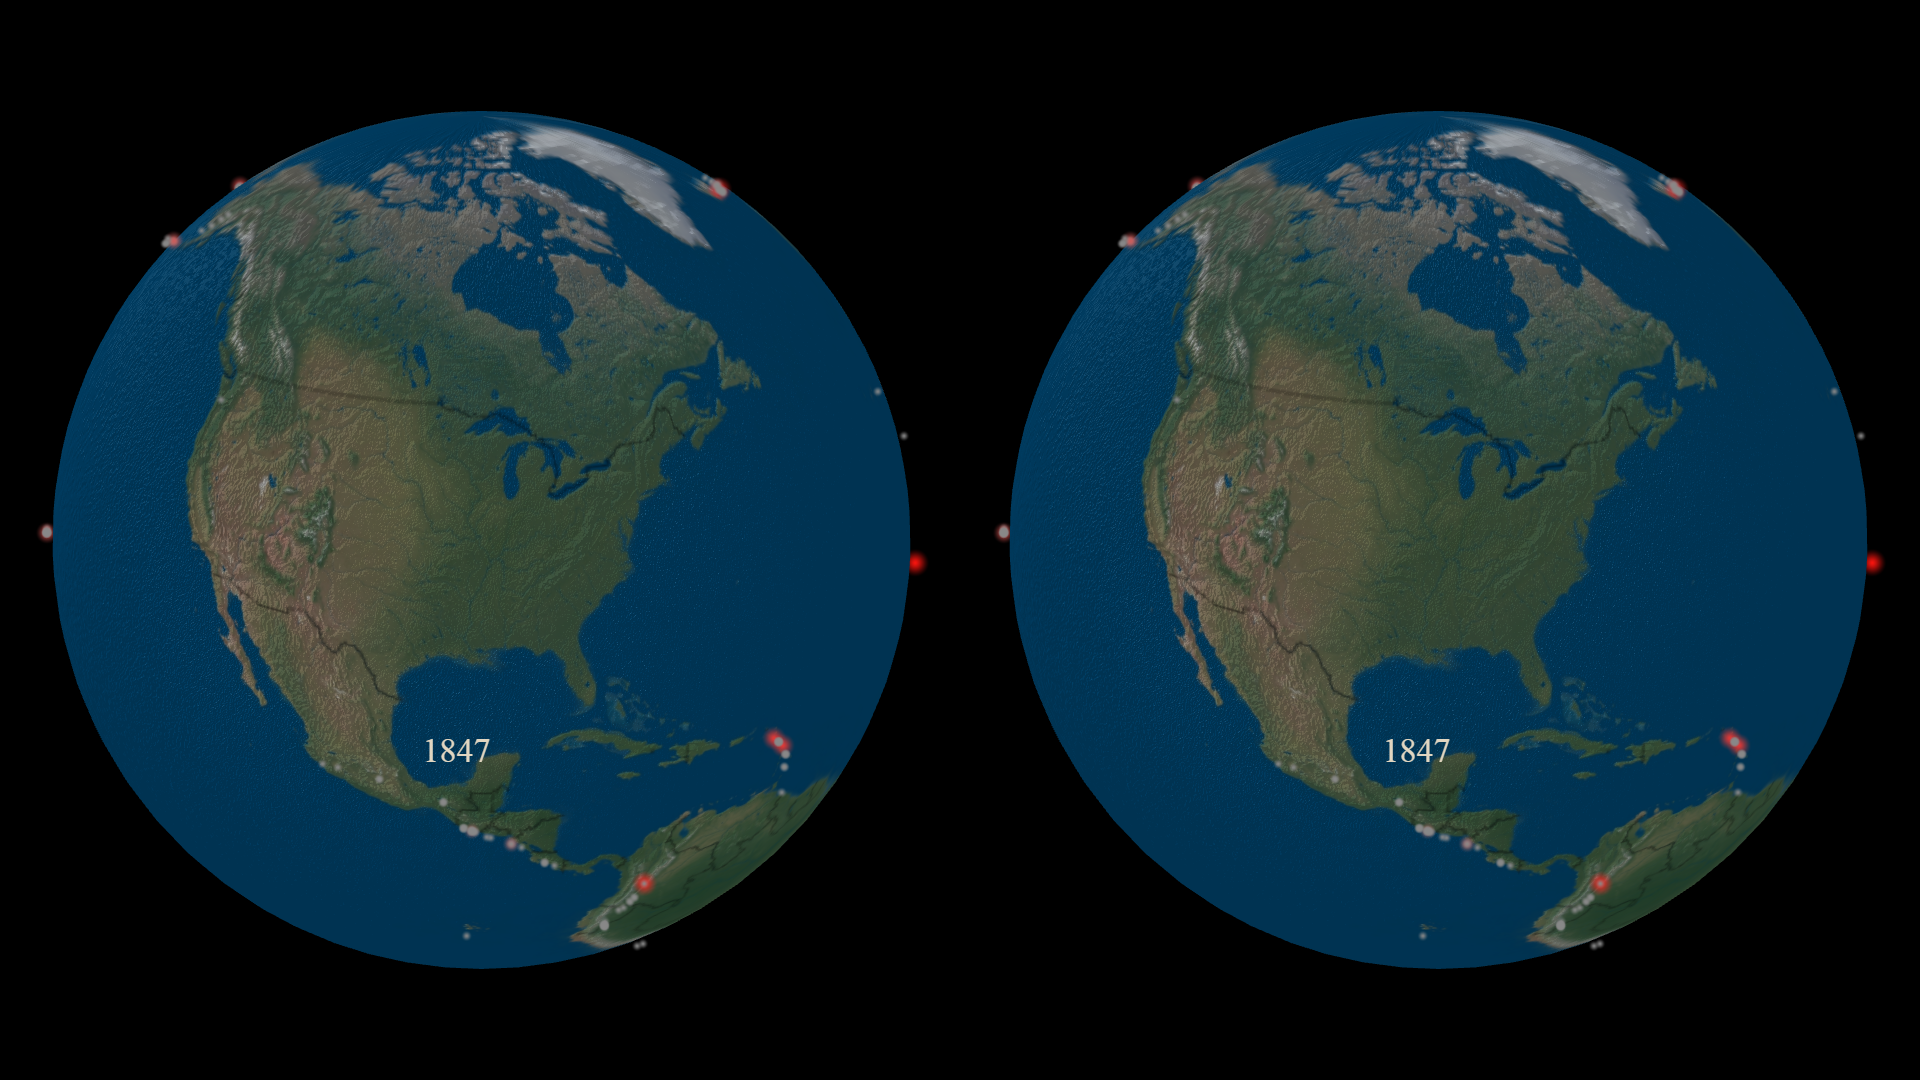
\includegraphics[width=3.4in]{images/vr}
  \caption{Fullscreen virtual reality mode using ``StereoEffect''}
\end{figure}

User interfaces in virtual reality are different from their traditional
counterparts, due to the level of engagement and differing input mechanisms.
Because of this, I increased the size of the date display and hid the time
slider, instead opting to autoplay through the time and loop around at the end.
When exiting from virtual reality mode, the standard controls return and the
visualization time is paused until further input is received.


\section{User Feedback}

I collected informal user feedback from classmates in Interactive Visualization
and from friends at RPI. Generally, users understood the purpose of the
visualization but had difficulty picking out and focusing on details. In
particular, it was confusing how many points were highlighted at the same time
for the location history data set.

Many users recommended incorporating map data, labels, or at least higher
resolution textures. While I wanted to connect to a map service, I felt that
this was out of scope for this project given the time provided. I was able to
find higher resolution textures and did not include a zoom option for the
virtual reality mode.

Initially, I faded the alpha value of particle images as they moved away from
the visualization time, which made it difficult to see trends in the data.
In response to this, I implemented HSV color and size interpolation.

A few users suggested hiding the Earth, making it transparent, or somehow
making data points visible through it. This was particularly relevant to the
volcanic eruptions dataset, since eruptions could be occurring on the opposite
side of the world and those points would not be visible.

\subsection{Follow Line}

To aid detail focus and point discovery, I drew a spline between the latest
data points in order. I called this a ``Follow Line'' (see Figure 7). As the
visualization time passed by a data point, that point was added to the line.
This served to connect points across time visually and could show when points
moved to the other side of the Earth.

This may have helped with the location history dataset, since those points
followed a clear chronological ordering, but the spline merely connected points
directly, so it could clip through the world. I am confident that I could
force the spline to follow a smooth path above the surface of the Earth, but
that will be left for future work.

After implementing this, I realized a critical difference between the location
history data and the volcanic eruptions data - volcanic eruptions are not
temporally related (in the sense that an eruption in one year should be
connected to an eruption in the next) while location history positions are.
Because of this, I disabled the ``Follow Line'' on the volcanic eruption dataset
and eventually dropped it from the location history dataset as well.

\begin{figure}
  \centering
  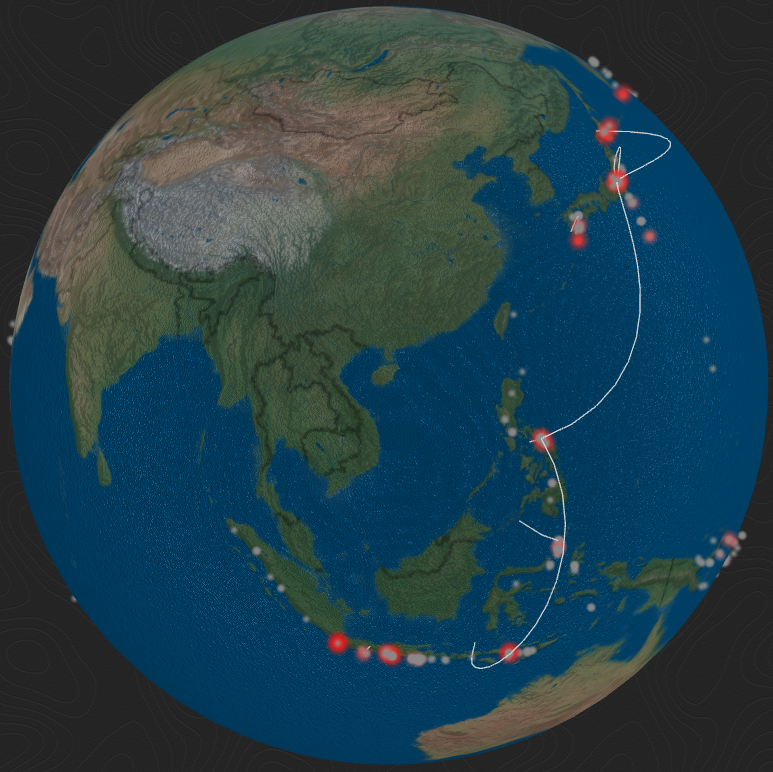
\includegraphics[width=3.0in]{images/follow_line}
  \caption{``Follow Line'' effect in use}
\end{figure}

\section{Limitations and Future Work}

There are several outstanding issues with the device orientation API, current
hardware, and my implementation on top of these technologies. As WebVR becomes
further developed, I would like to transition over to that.

I would also like to integrate map data from a provider like Google Maps or
OpenStreetMap, since my current implementation handles zooming very poorly and
provides little cultural context to the raw geography present in the Earth
textures used.

I did not test on an Oculus Rift or any virtual reality device other than the
Google Cardboard, so that is an obvious path for future work to ensure
compatibility. Perhaps the larger display and more precise motion tracking on
the Oculus Rift would solve several of my issues there.

Now that I have a working virtual reality globe capable of displaying geographic
time series data, I feel that I should re-evaluate the usefulness of this
interface and investigate if there are other interactions relating to this setup
which would aid in data analysis. Future visualization design could either
center on overview information and trends or on specific detail focus. I think
that virtual reality will eventually be great for specific detail focus and
exploration, but trend viewing might be easier to reach at the moment.

\section{Conclusions}

I have built an interactive virtual reality visualization of geographic
location history data and applied this visualization to both my personal
location history data as well as volcanic eruption history data.

While the interface and interaction were both interesting, details were
difficult to notice and several technical limitations held the project back.
Shifting from using both d3.js and three.js to using only three.js was a great
decision and solved a number of implementation challenges. There is hope that
WebVR will smooth out the remaining device orientation issues.

\bibliographystyle{acmsiggraph}
\bibliography{chronographer}
\end{document}
